\section{\ArchName Network Management}
\label{sec:system}

In this section, we focus on the design of a {\em datacenter
  management layer} that uses building blocks from previous sections,
to implement a \blue{feasible} reconfigurable datacenter network.
%
We start with describing the high-level roles of the different
components of the management layer. See Figure~\ref{fig:mgmt}.

\begin{wrapfigure}{r}{0.5\textwidth}
\vspace{-1cm} 
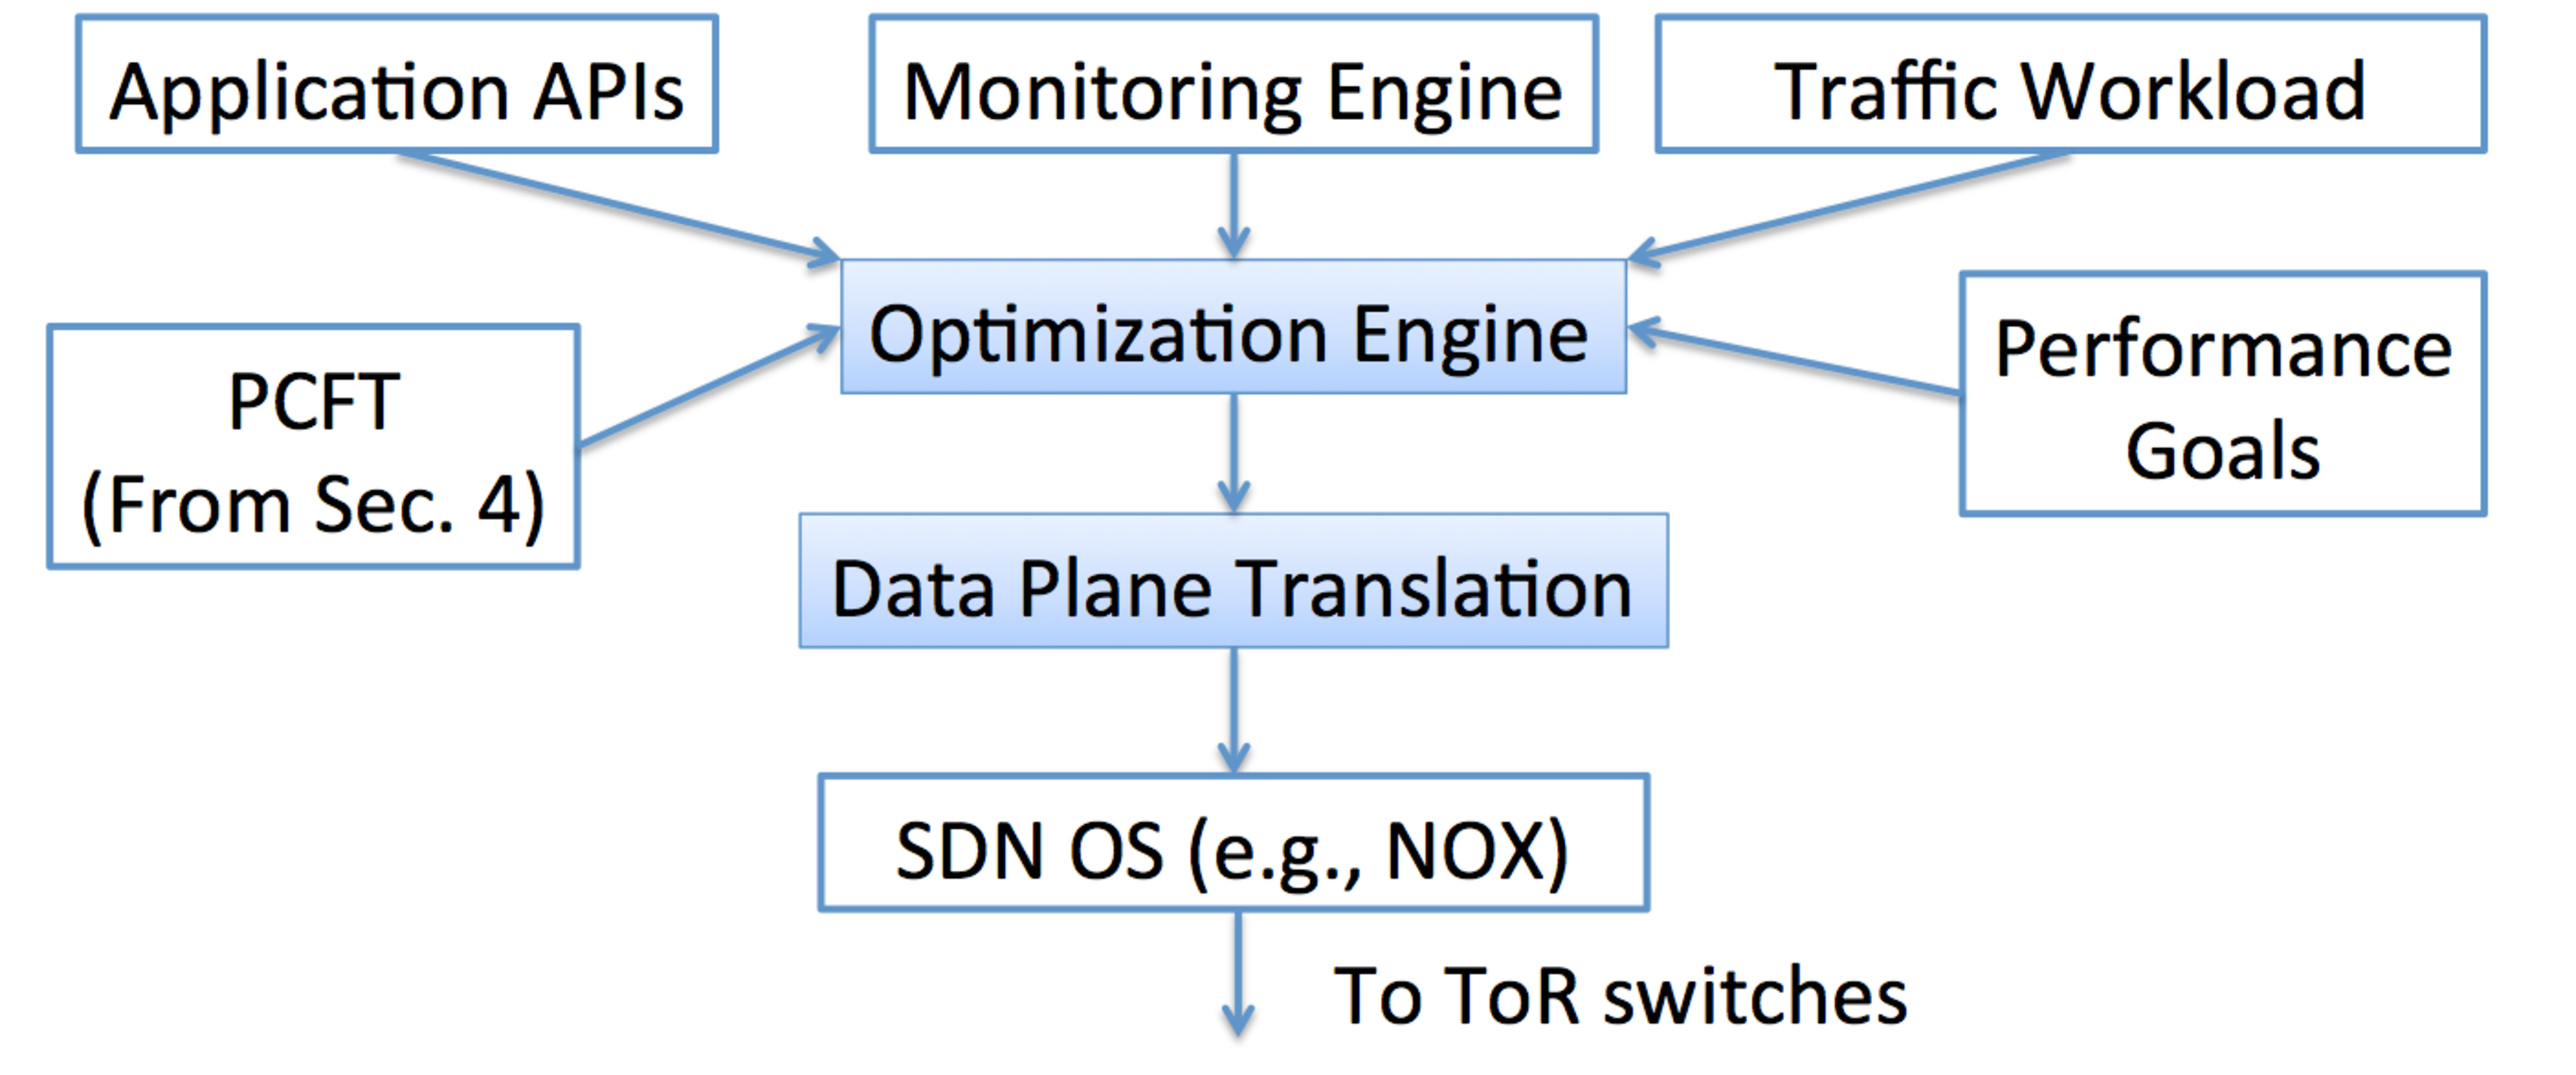
\includegraphics[width=240pt]{PPTFigs/sysoverview-new.pdf}
\vspace{-0.8cm} 
\caption{Overview of the \ArchName management layer}
\vspace{-0.6cm} 
\label{fig:mgmt}
\end{wrapfigure}

\begin{packeditemize}
\item {\bf Monitoring Engine (ME):} ME provides network status
  information (e.g., links status, traffic patterns, or views
of ``elephant'' flows~\cite{hedera,devoflow,conext13ericson})
to the management layer. 

\item {\bf Optimization Engine (OE):} Given the offered traffic
  workload, a pre-configured flexible topology (PCFT), and the current
  network state (e.g., link status), the optimization engine devises
  an efficient {\em reconfiguration and traffic engineering strategy}
  so as to optimize desired performance goals.

\item {\bf Data Plane Translation Engine (DPE):} DPE translates the
  OE output into an efficient data plane strategy.

\item {\bf Application APIs:} APIs enable the users/tenants to inform
    application details (e.g., expected traffic patterns,
    single/multi-path TCP) to the optimization and data plane modules,
    \blue{to best leverage the benefits of \ArchName.}
\end{packeditemize}

\softpara{Plan.} For the ME, we will leverage past work on scalable 
traffic matrix and elephant flow
detection~\cite{hedera,devoflow,yingzhangconext13}.  Similarly, we
will extend prior work on APIs for applications to expose traffic
patterns~\cite{coflow,bigdatahotsdn}.
%
We address OE and DTE in the following subsections. In the last
subsection, we address design of a wireless out-of-band control
network for configuration dissemination and data collection.

\subsection{Reconfiguration and Traffic Engineering}
\label{sec:reconfig}

\begin{task}
\label{task:system:fastalgo}
We will develop fast and efficient algorithms for the joint
optimization problem of reconfiguration and traffic engineering.
\end{task}

%To explain the optimization problem that we
%need to solve and highlight why this problem is hard, we begin with an abstract
%integer linear program formulation in a static setting.

\para{Joint Reconfiguration and Traffic Engineering (JRTE) Problem.}
Given the traffic load, the {\em JRTE} problem is to: (a) Select a
realizable-topology from a given pre-configured flexible topology
(recall that a realizable-topology is a matching of candidate links
over the FSOs); and (b) Route the given inter-rack flows over the {\em
  selected} realizable topology, so as to optimize a desired
objective. The second traffic engineering (TE) part essentially
involves solving the multi-commodity flow problem over the realizable
topology.  \blue{For the latter, the set of FSOs on each rack are
  considered as one node (since they are connected by a ToR switch).}
%
The objective functions of interests could be to minimize link
congestion or maximize total flow in conjunction with fairness,
latency bound, and/or tenant provided SLAs.

\para{Connection to Prior Works} For the special case when the given
PCFT has exactly one realizable-topology (i.e., the given candidate
links already form a matching over the FSOs), our JRTE problem is
exactly the NP-hard~\cite{} multi-commodity flow problem with the
desired objective, \blue{assuming the given TCP flows to be
  unsplittable~\cite{hedera}.} Thus, our JRTE problem is trivially
NP-hard.
%
The reconfiguration subproblem can be looked upon as a kind of
topology control problem~\cite{}, which is to establish/select links
between given wireless nodes to achievenetwork connectivity while
minimizing the transmission power (or energy consumption) of the
nodes. The constraints and objectives of the topology control problems
are quite different than our reconfiguration subproblem, and thus, the
techniques used for topology control are not directly applicable.
%
Finally, the reconfiguration subproblem (as the PCFT problem) also
falls in the class of {\em degree-constrainted subgraph} problem, but
the TE-based objectives makes the reconfiguration subproblem very
different from prior-addressed degree-constrainted subgraph problems.

\para{Proposed Approaches.} We note that the ILP formulation of the
JRTE problem took several hours to solve on the state-of-art ILP
solver~\cite{}, even for a small 20-node instance. In contrast, the
reconfiguration of our \ArchName network should not take more than a
few milliseconds, for it to be of any real benefit. Thus, the
challenge is to design very fast, scalable, and efficient JRTE
algorithms.

\begin{packeditemize}
\item {\em Matching Techniques.} One simple and reasonable way to
  approach the reconfiguration subproblem would be to select the
  maximum-weighted matching (solvable in polynomial time) between
  FSOs, where the link $(i,j)$ is weighted by the inter-rack traffic
  demand between the correspondin racks. Such a topology essentially
  serves the maximum possible total inter-rack demand using {\em one}
  hop paths.  It is challenging to generalize the above approach to
  include two-hop routes, i.e., to select the matching that serves the
  maximum traffic demand in one or two hops. In general, we would like
  to pick a matching that yields the minimum weighted average
  inter-rack distance (where the distances are weighted by the traffic
  demands). Even generalizing the matching algorithm to ensure that
  the corresponding inter-rack graph is connected is challenging, but
  this may be a reasonable tractable objective. \blue{After picking a
    matching, we can do the TE part independently using standard
    techniques~\cite{} over the selected topology.}

\item {\em LP Relaxation Techniques.} One promising approach is to
  formulate the reconfiguration problem as an ILP (using flow-like
  constraints and binary variables for link selection) with the
  objective of minimum link congestion or maximum total ``fair''
  flow~\cite{max-fair-flow}, and solve the relaxed LP. We can then
  convert the LP solution to an ILP solution by an appropriate
  ``rounding'' technique, while ensuring that the ``matching
  constraint'' is still satisfied (unsatisfied flow-constraints will
  only result in a sub-optimal TE solution). \blue{Here, for the
    unsplittable (i.e., single-path routing) verion, we also need to
    do path-striping as in~\cite{rand-round} in conjunction with the
    rounding process.}  An alternate approach in a similar vein as
  above is: First solve the multi-commodity flow problem over the
  entire PCFT graph, and then select a ``good'' matching based on the
  flow values on the links. Both above approaches are expected to be
  fast, and it would be interesting to compare their relative
  performance over real traffic traces.
\end{packeditemize}

\para{Further Directions.} In addition to the above, we are also
interested in designing algorithms based on limited traffic
information, and incremental or localized approaches.

\begin{packeditemize}
\item {\em Strategies with Limited Traffic Information.}  Our previous
  discussion implicity assumes availability of traffic demands for the
  next \blue{epoch.}  However, in reality, traffic predictability may
  be limited. In the worst case, we may only be able to distinguish
  between ``elephant'' (large) and ``mice'' (small) flows, based on
  their \blue{initial size.}  In such restricted settings, the
  reasonable approach would be to change the \blue{realized topology}
  in an ``online'' manner in response to the arriving elephant flows,
  while relying solely on TE for the mice flows. This approach should
  be effective since the structure of real-world workloads suggests
  that a small number of elephant flows carry the most
  bytes~\cite{}. Moreover, since these elephant flows are typically
  long-lived~\cite{}, they are quite amenable to coarser time-scale
  optimizations. In our preliminary work~\cite{hotnets}, we employed a
  simple strategy along the above directions, and achieved
  near-optimal performance over randomly generated traffic
  traces. \blue{More information about traffic loads such as spatial
    and temporal distribution of elephant flows (or flow sizes in
    general) would require challenging generalizations of the above
    approach.}

  An addition challenge to address in the above online strategy would
  be to favor JRTE solutions that cause minimal disruption to existing
  traffic flows. In general, we would like to be able to estimate the
  {\em overall impact} (including, disruptions to current flows and
  in-flight packets) of a possible JRTE solution, and only suggest
  solutions whose overall impact is beneficial. We could define the
  {\em impact} in terms of the expected change in average evacuation
  time, packet latency, and/or number of dropped packets. Computation
  of such appropriately defined impact may be intractable, but upper
  and/or lower bounds on its value may be sufficient and very useful
  for our purposes.

\item {\em Incremental or Localized Strategies.} One of the ways to
  develop a fast and effective JRTE algorithm is to determine the
  solution in an incremental manner (e.g., by constraining the number
  of links that need to deactivated or activated), and morever, even
  limiting ourselves to only localized (i.e., close to where the
  traffic changes occur) strategies. To design incremental JRTE
  algorithms, we can use augmenting-path techniques to incrementally
  improve the matching~\cite{}, with additional constraints and/or a
  modified objective function. For localized strategies, we can
  exploit the flow structure of the optimization to design distributed
  strategies~\cite{khandekar,conext13}. Note that localized
  reconfigurations may result in multiple {\em concurrent}
  reconfigurations across the network, which would need to be handled
  carefully to ensure \blue{consistency and connectivity} (as
  discussed in the next subsection).
\end{packeditemize}

\eat{
First, we simplify the traffic engineering aspect of the problem by
aggregating the given inter-machine flows into inter-rack flows, and
allowing the aggregated inter-rack flows to be splittable (across
multiple paths.)  Such a simplification makes the traffic engineering
problem much easier (splittable multi-commodity flow problem is in P),
while allowing the split inter-rack flows to be mapped to non-split
original TCP flows using ``path-striping''~\cite{}; such a mapping
should work well for most practical inputs.}

\subsection{Data Plane Strategies}

\begin{task}
\label{task:system:dataplane}
We will design and implement efficient data-plane implementations to
guarantee \blue{reachability and consistency properties}, in presence
of reconfiguration and link dynamics.
\end{task}

\smallskip

In translating the JRTE solution into a consistent and efficient data
plane forwarding strategy, we build upon recent advances in
software-defined networking (SDN), as it provides cleaner management
abstractions and open interfaces (e.g., via APIs such as
OpenFlow~\cite{}). However, \ArchName introduces unique challenges.
In particular, in face of a dynamically changing network due to
reconfigurations, we need to ensure that: (a) packets do not use
deactivated links \blue{(i.e., black holes~\cite{} are avoided)}, (b)
the network remains connected at all times, and (c) the packet latency
remains bounded. Finally, we also need a data plane strategy to: (d)
handle transient misalignment of FSO links. We note that the recent
related works either assume a {\em static}
network~\cite{cons-update,incconsupdate} or focus on a single
reconfiguration~\cite{cu-1}, and hence, are not directly applicable to
our context.

\para{\underline{(a) and (b).} Avoiding Black Holes, and Guaranteeing
  Connectivity.}  Packets are routed in the network on the basis of
forwarding tables, which essentially specify, at each node, the next
hop/link to use for each destination. In a dynamic network, forwarding
tables will also be changing constantly.  Note that
activation/deactivation of a link \blue{may take a few tens of msecs,
  and that we cannot directly update the tables across all the network
  switches in one atomic action.}
%
In face of these challenges, we need to ensure that through every
possible intermediate state of the switches' tables and links, the
forwarding tables always refer to only active links. We can ensure
this by a careful ordering of steps as suggested in our preliminary
work~\cite{hotnets}. In particular, (i) we reflect removal of links in
the forwarding tables, before actually deactivating the links, and
(ii) reflect addition of links in the tables only after the link
activation is complete. The above solution works irrespective of the
order in which the forwarding tables are updated across the network,
and even in the presence of multiple concurrent reconfigurations. 

In addition to above, we also need to ensure that the network remains
connected at all times. There are two possible solutions to this: (i)
maintain a static ``backbone'' subnetwork that ensures connectivity,
or (ii) reject reconfigurations that disconnect the network. The first
approach reduces the degree of flexibility in network design and
\blue{could result in poor performance.} The second approach requires
a careful implementation if there are multiple {\em concurrent}
reconfigurations. Concurrent reconfigurations can be handled in three
ways: (i) one at a time, (ii) in batches (i.e., queue and combine them
into a single reconfiguration); and (iii) execute each reconfiguration
individually but {\em concurrently}. The first two options introduce
unnecessary reconfiguration delays, while the third option requires a
careful implementation to ensure correctness---we need to keep a
single consistent view of the network topology graph and allow only
{\em atomic} access to it (when checking if a reconfiguration
disconnents the network). \eat{Again, the above solutions work
  irrespecitve of the order in which the forwarding tables are updated
  across the network.} In our research, we will study and compare the
performance of such approaches.

\begin{wrapfigure}{r}{0.3\textwidth}
\vspace{-0.4cm}
\centering
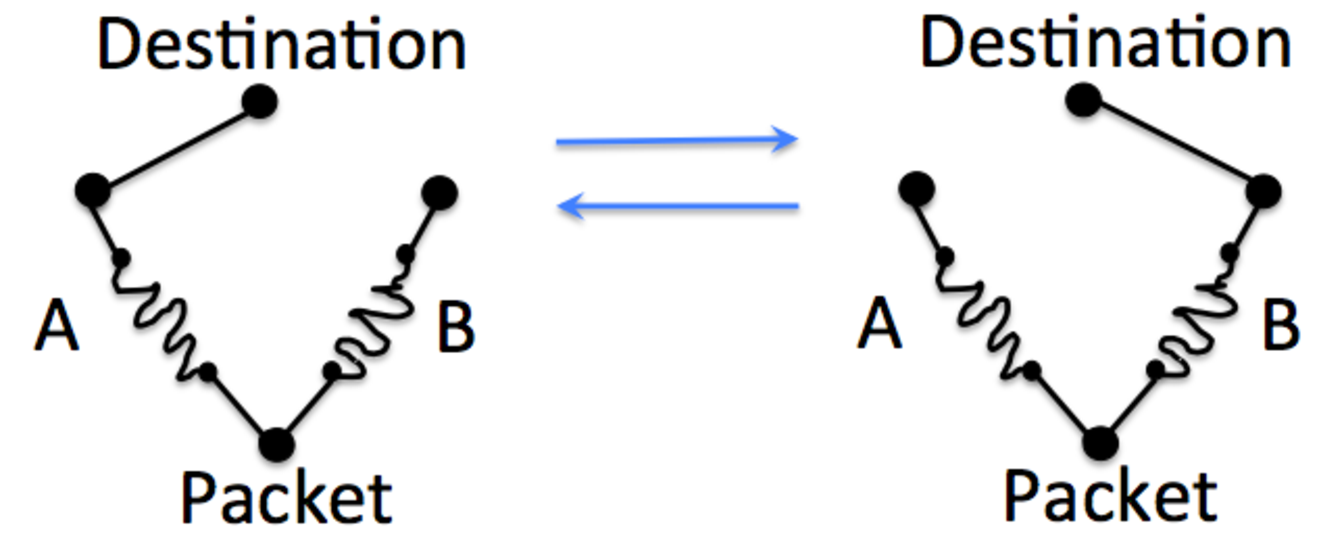
\includegraphics[width=150pt]{PPTFigs/impossible.pdf}
\caption{If the network goes back and forth between the above
  topologies (due to corresponding reconfigurations), then the packet
  will continue to ``swing'' between areas A and B---leading to a
  (perennial) forwarding ``loop''.}
\label{fig:impossible}
\end{wrapfigure}
\para{\underline{(c)} Guaranteeing Bounded Packet Latency.}  The above
strategies still do not guarantee a bounded packet latency. In fact,
in general, its {\em impossible} to guarantee bounded packet latency
(e.g., see Figure~\ref{fig:impossible}). 
%
However, such situations can be avoided if we ensure a minimum time
interval between consecutive reconfigurations; this minimum interval
is also essential for the centralized controlled and the wireless
control channel to be able to handle the resulting load (see
Section~\ref{sec:wireless}.)  In particular, we can formally prove
that a minimum interval of $(x + y)$ time units between
reconfigurations suffices to ensure an upper bound of $2x$ units on
packet latency, where $x$ is the bound on packet latency given a fixed
network and $y$ is the maximum time taken to update (not necessarily
atomically) the network forwarding tables.
%
We can expect $x$ and $y$ to be of the order of 1-2 msecs. Note that
the above claim is independent of the link activation or deactivation
latency (which can be a few tens of msecs).

\para{\underline{(d)} Handling Misalignment of Links.} In \ArchName,
even during a static topology state, links may be temporarily
unavailable because of possible misalignment of the FSO
links. \blue{Such misalignments are fixed in real-time by mechanisms
  suggested in Section~\ref{sec:fso}} in timescales much smaller than
the time needed to update rules~\cite{ddcnsdi13} by an SDN
controller. In fact, it may even be counterproductive to report such
transient link failures to the controller, as it may cause needless
update of forwarding tables. Thus, we need appropriate \blue{network
  layer} techniques to recover from such transient link
failures. \blue{Future SDN roadmaps have provisions for local recovery
  mechanisms analogous to similar schemes in the MPLS and SONET
  literature~\cite{}. We will explore the available alternatives in
  our research. In the absence of such features,} we will investigate
design of a local ``lightweight'' SDN controller on every rack that
can quickly react to such misalignments.

